



\documentclass[a4paper,12pt,spanish]{article}

\usepackage[utf8]{inputenc}


\usepackage{blindtext}
%\usepackage{microtype}
\usepackage{amsfonts, amsmath, amsthm, amssymb}
%\usepackage{fancyhdr}
%\usepackage{index}
%\usepackage{multicol}    

%\usepackage{booktabs}

\usepackage[T1]{fontenc}
\usepackage[utf8]{inputenc}
\usepackage{graphicx}
\usepackage[spanish,es-tabla]{babel}
\usepackage{url}
\usepackage{enumitem}

\usepackage[unicode=true, pdfusetitle,
bookmarks=true,bookmarksnumbered=false,bookmarksopen=false,
breaklinks=true,pdfborder={0 0 1},backref=false,colorlinks=false]
{hyperref}

\usepackage{listings}
\usepackage{longtable}


\usepackage{siunitx} %para el sistema internacional
\usepackage[export]{adjustbox}
\usepackage{booktabs} 
\usepackage{subcaption}

\usepackage{float}


\newcommand{\address}[1]{
	\par {\raggedright #1
		\vspace{1.4em}
		\noindent\par}
}

\usepackage[table,xcdraw]{xcolor}


\pagenumbering{gobble}
\include{noNumberPage}
\pagenumbering{arabic}
\setcounter{page}{1}

%tutorial de tablas latex: https://manualdelatex.com/tutoriales/tablas

\usepackage{multirow}

% \usepackage[table,xcdraw]{xcolor}


%Inicio del documento (hasta que se cierre con \end{document}
\begin{document}
	
	
	\title{ Espectroscopía Gamma con detectores de INa(Tl) }
	
	
	%\author{Adrián Rivero Fernández}
	\date{}
	
	\maketitle
	
	
	\section{Objetivos de la práctica}
	
	\vspace{\baselineskip}
	
	1. Medir el fondo radiactivo con el detector cerrado y abierto.\\
	
	2. Calibrar en energías con una fuente radiactiva.\\
	
	3. Determinar la eficiencia del detector, medirla para varias energías y graficar la eficiencia en función de la energía.\\
	
	4. Medir la resolución de diferentes picos y graficar la resolución en función de la energía.\\
	
	5. Estudiar los espectros, determinar teórica y experimentalmente el fotopico, la distribución de Compton y la retrodispersión de cada espectro.\\
	
	6. Determinar la actividad de la muestra de actividad desconocida.\\
	
	7. Determinar las energías de una muestra desconocida. Determinar su composición.\\
	
	
	\section{Determinación del fondo}
	
	
\begin{figure}[H]
	\centering
	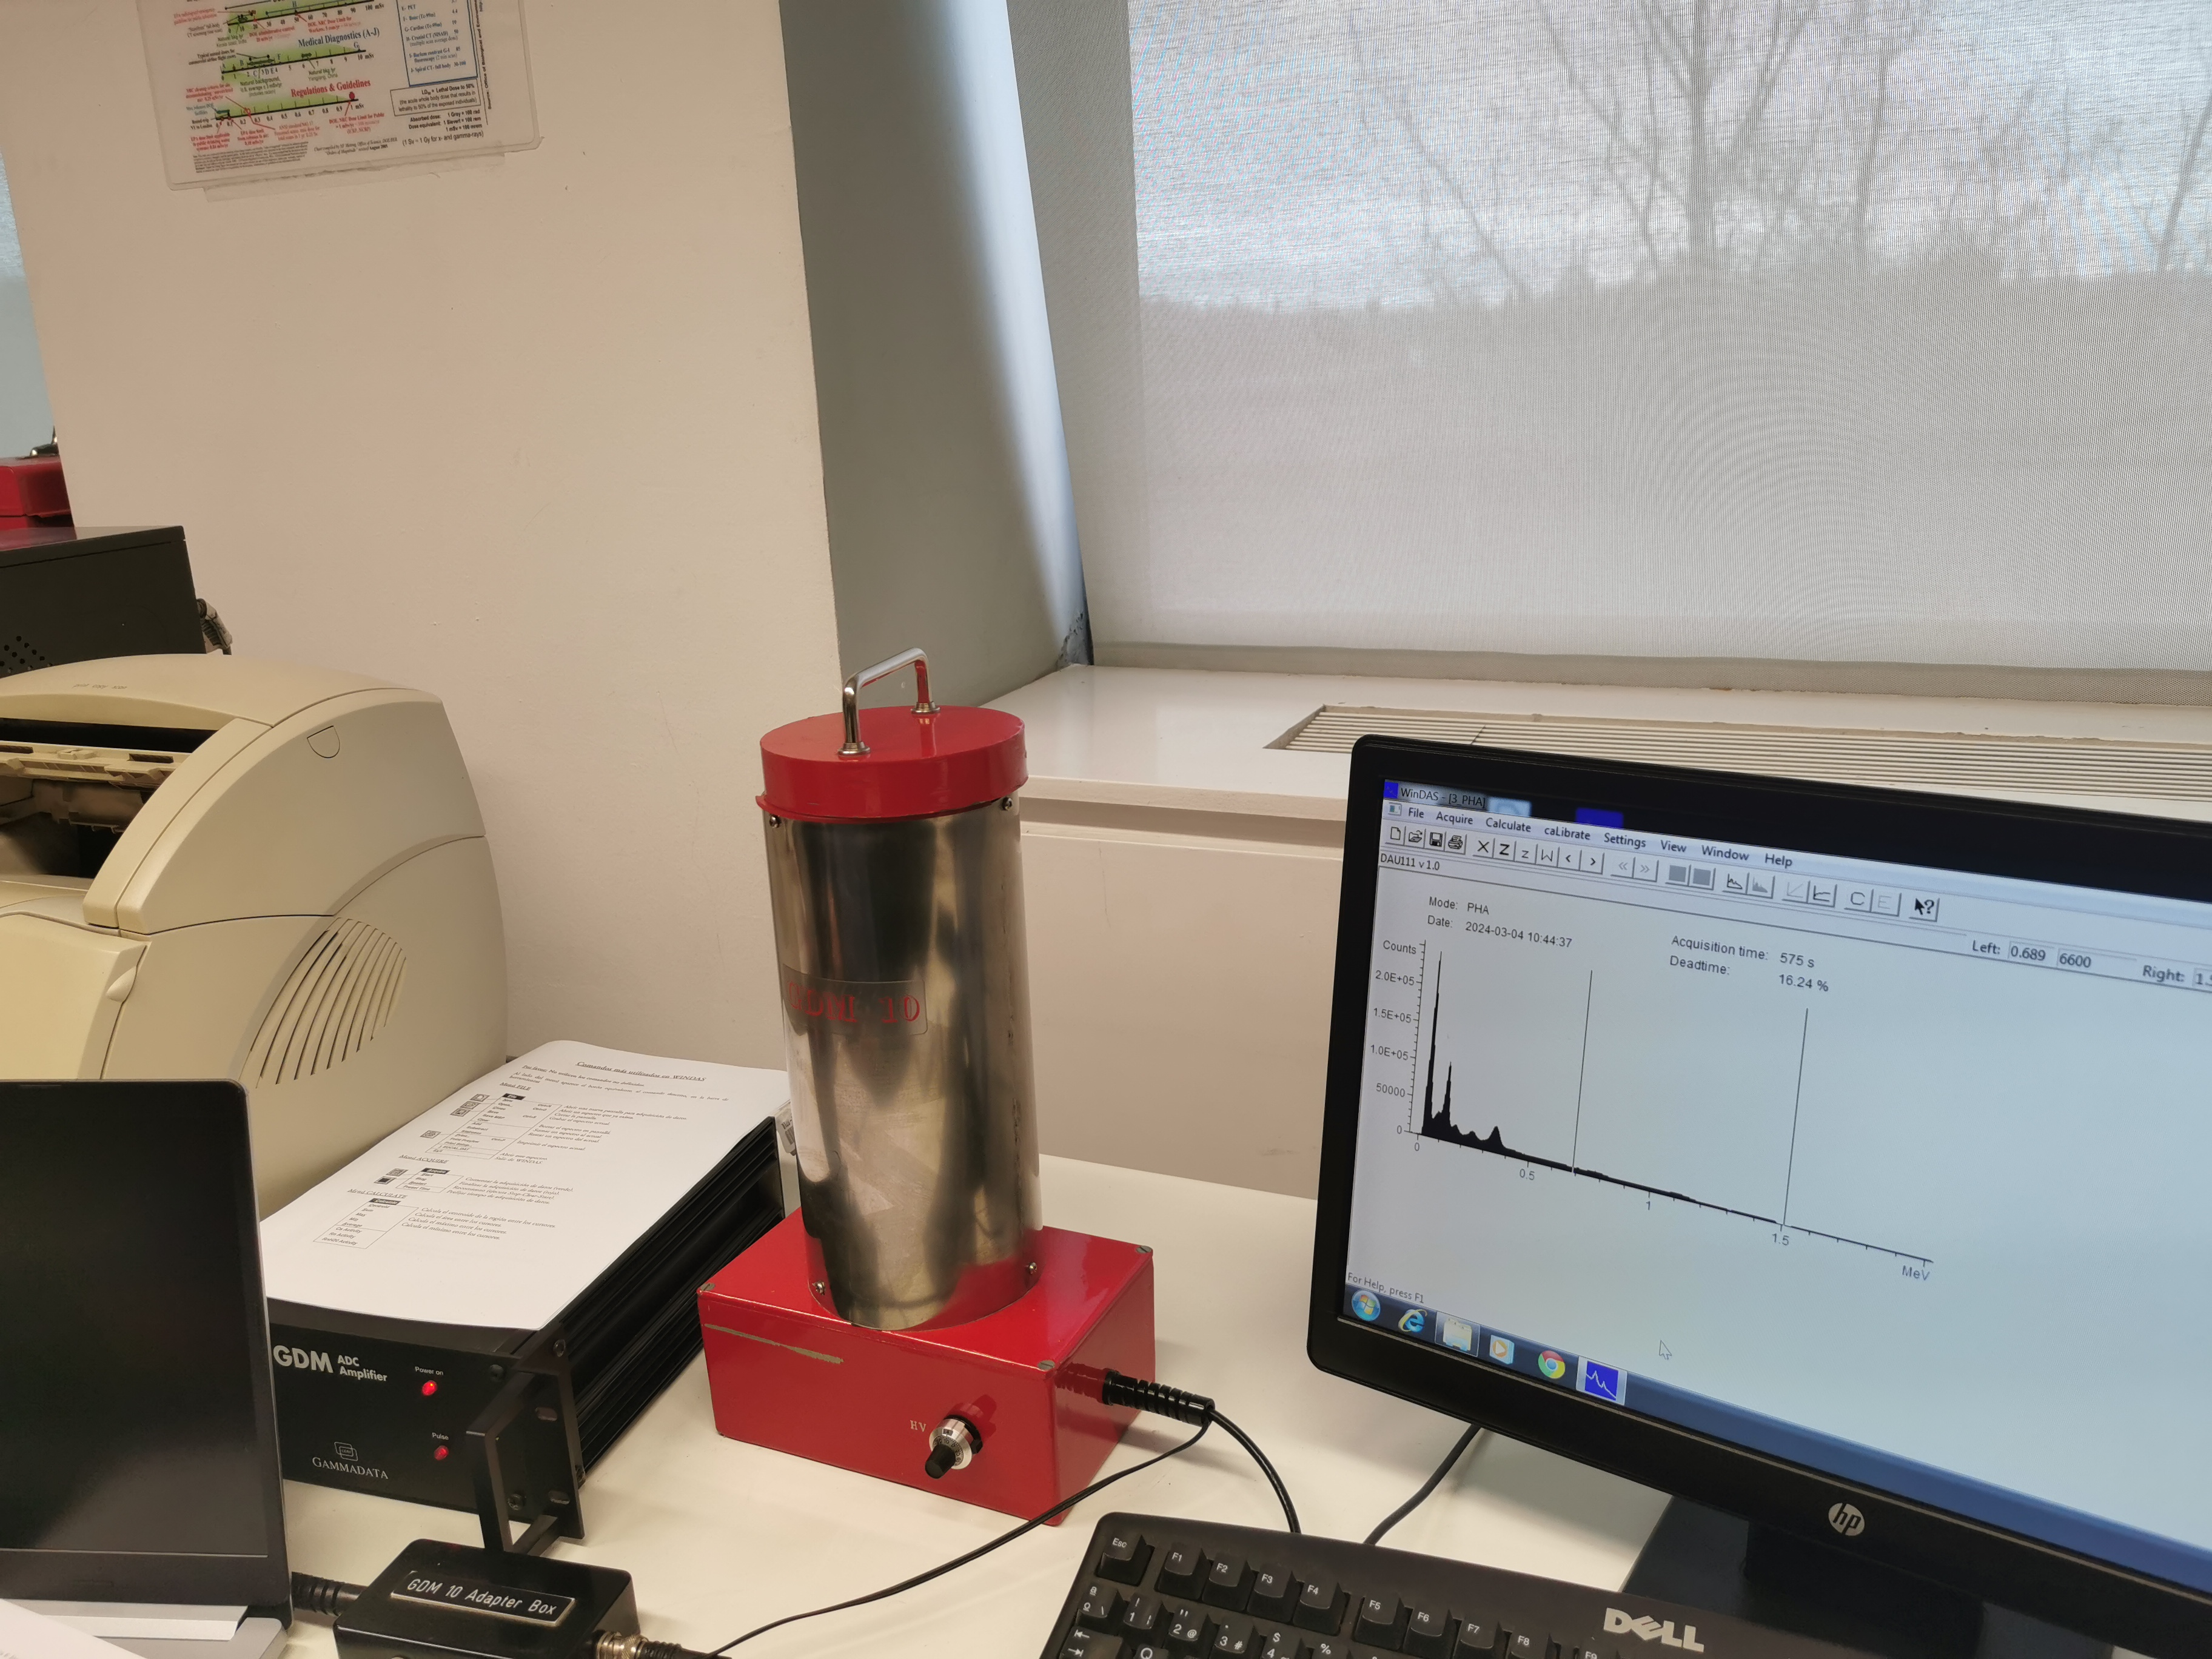
\includegraphics[width=0.7\linewidth]{../IMG_20240304_110653}
	\caption{Detector con su sistema de digitalización.}
	\label{fig:img20240304110653}
\end{figure}

	Iniciamos los aparatos, y tomamos muestras del espectro del fondo con el castillete vacío tapado y destapado.
	
	
\begin{figure}[H]
	\centering
	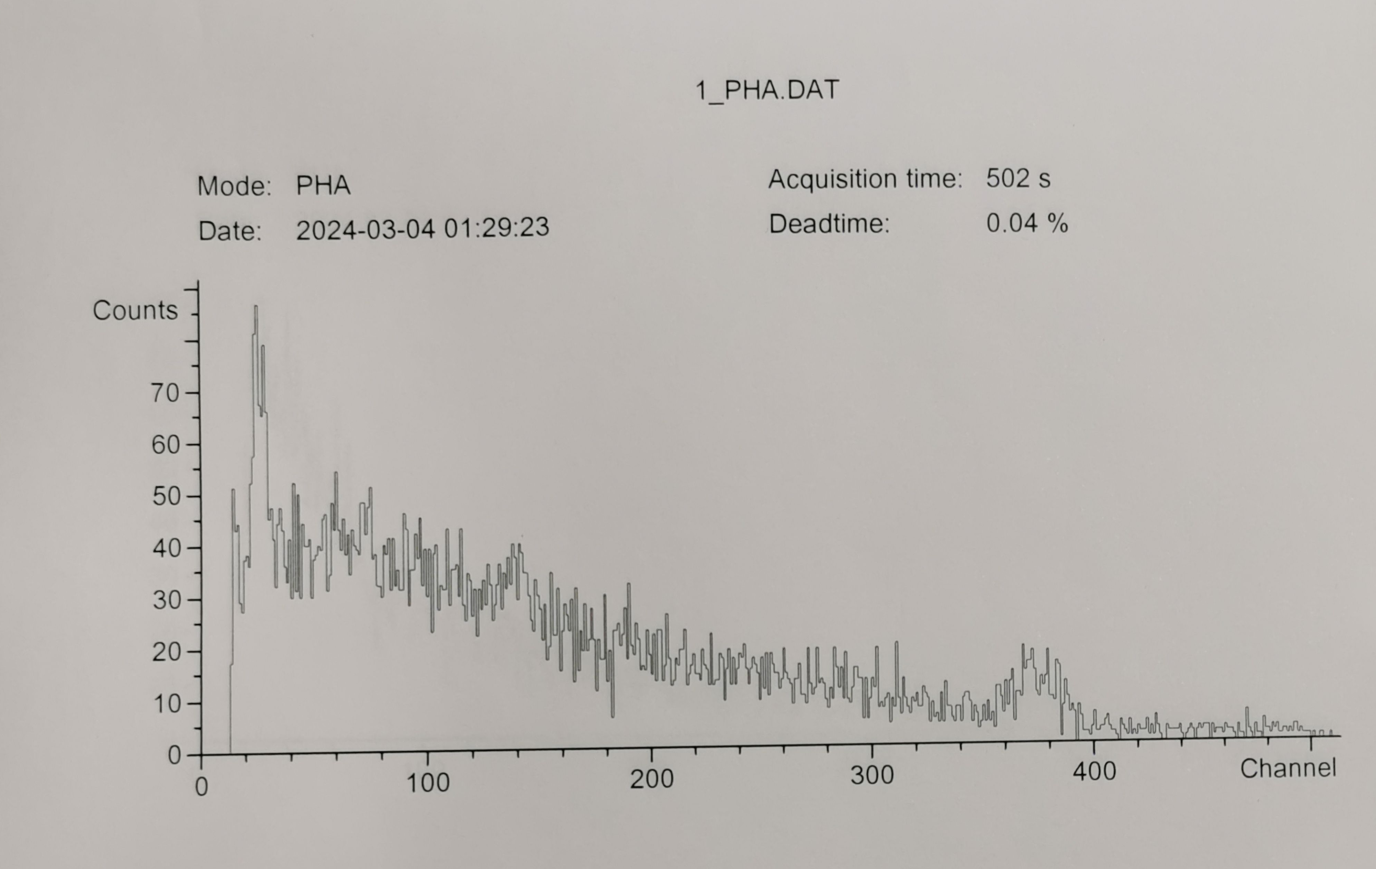
\includegraphics[width=0.7\linewidth]{../graficas_procesadas/PHA_1}
	\caption{Medición de fondo con el castillete tapado}
	\label{fig:pha1}
\end{figure}
	
	
\begin{figure}[H]
	\centering
	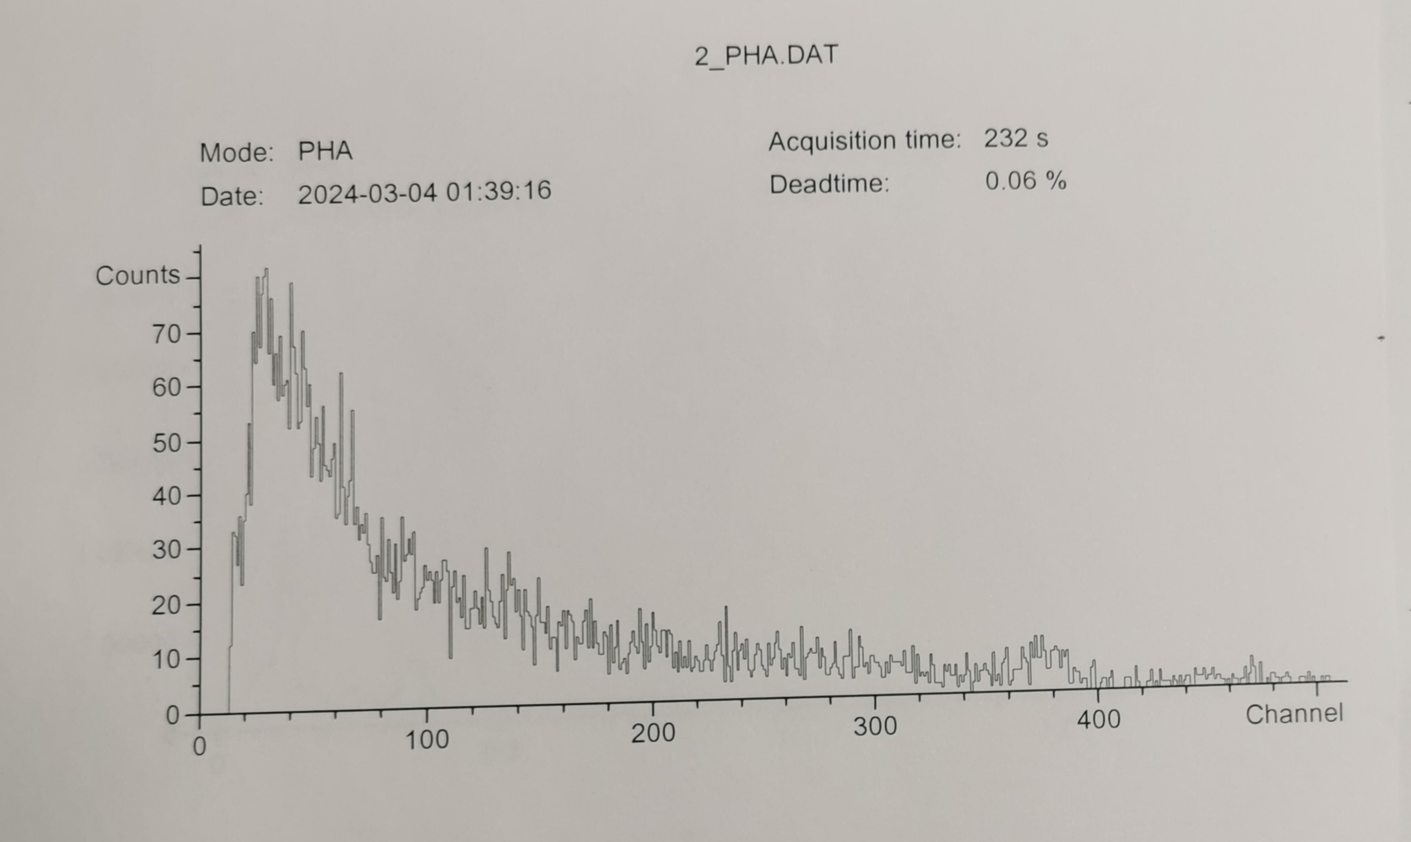
\includegraphics[width=0.7\linewidth]{../graficas_procesadas/PHA_2}
	\caption{Medición de fondo con el castillete destapado}
	\label{fig:pha2}
\end{figure}



%%%
% [[Qué se puede deducir del fondo con el detector cerrado y abierto?]]
% [[Es necesario tener en cuenta el fondo del detector en las medidas?¿Por qué?]]
 
 
 El espectro es similar en ambos casos, presentando un bajo conteo de radiación con un pico en las bajas energías, que es más ancho con la tapa destapada. Podemos deducir que el pico en bajas energías probablemente se deba a la radiación gamma ambiental, mientras que la diferencia en el ancho del pico sugiere que hay más radiación gamma de baja energía alcanzando el detector cuando está destapado, lo que puede deberse a fuentes adicionales de radiación cercanas.
 
 Es necesario tener en cuenta el fondo del detector en las medidas para no malinterpretar la radiación de las muestras, que se verán afectadas por el fondo. 
 
 
	
	\section{Calibración de energías}
	
	
	
	Tomamos primero el Europio-152, que usaremos para calibrar el detector. El espectro de radiación $\gamma$ se trata de un espectro contínuo, como podemos ver, ya que los fotones gamma se generan con una amplia variedad de energías, en lugar de valores discretos.
	
	
	
\begin{figure}[H]
	\centering
	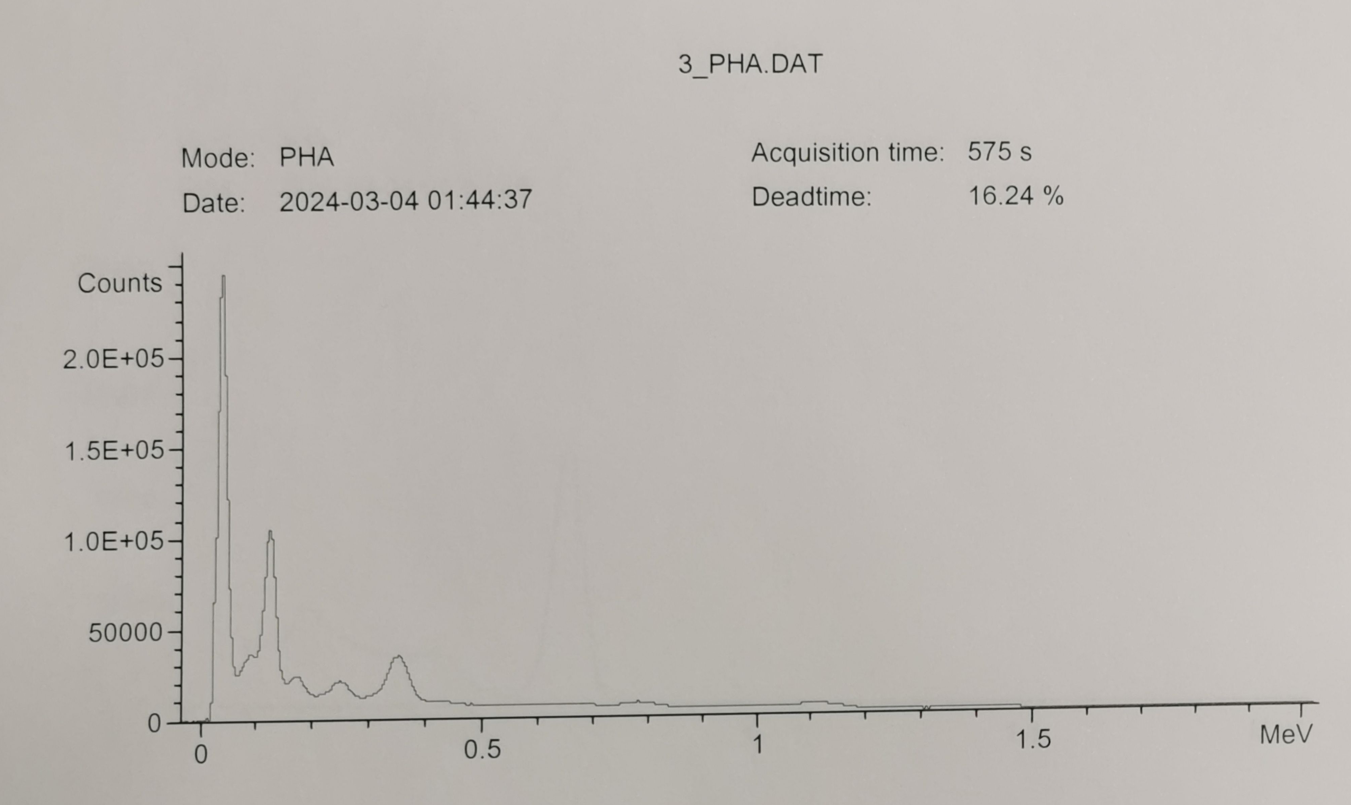
\includegraphics[width=0.7\linewidth]{../graficas_procesadas/PHA_3}
	\caption{Espectro gamma del Europio-152}
	\label{fig:pha3}
\end{figure}
	
	\subsubsection*{1º pico: 0,122 MeV}
	Centroide = 38,97
	
	\subsubsection*{2º pico: 1,41 MeV}
	Centroide = 359,56
	
	\vspace{\baselineskip}
	
	Con estos datos, calibramos y comprobamos el resto de picos del Eu$^{152}$. \\
	
	La calibración es esencial ya que nos permitirá comparar mejor los espectros de diferentes muestras, identificar picos con mayor facilidad y corregir desviaciones experimentales.
	
	
	
	\section{Eficiencia del detector para las gammas}
	
	Primero calculamos la actividad real de la muestra, teniendo en cuenta que la actividad inicial a 12 de octubre de 2022 era de 1$\mu$Ci, a día 4 de marzo de 2024 (1 año y 5
	meses después):
	\[ A = A_0 \text{e}^{-\frac{\ln2}{T_{1/2}t}}\]
		
	con 
	
	\[A_0 = 1\si{\mu Ci}\]
	\[t = 1,42 \text{años}\]
	\[ T_{1/2} = 13 \text{años}
	\]
	Quedando
	\[ A = 0,927\si{\mu Ci} = 34308,14 \si{Bq}
	\]
	
	Teniendo en cuenta la relación entre la actividad y la eficiencia
	\[ A = \frac{A_f}{\varepsilon(E) C_r} \longrightarrow \varepsilon = \frac{A_f}{A·C_r}
	\]
	siendo $A_f$ el area del fotopico en Bequerelios, $A$ la actividad calibrada, $\varepsilon$ la eficiencia y $C_r$ el coeficiente de ramificación (dado en el guión de prácticas) correspondiente a cada pico.
	
	\begin{table}[H]
		\centering
		\begin{tabular}{|c|c|c|c|c|c|}
			\hline
			$E$ (MeV) & $E$ real (Mev) & $A_f$ (Bq) & Cr    & Eficiencia $\varepsilon$ & $\varepsilon$(\%) \\ \hline\hline
			0,04      & 0,039          & 2113       & 0,567 & 0,108      & 10,807          \\ \hline
			0,122     & 0,122          & 806        & 0,307 & 0,076      & 7,613           \\ \hline
			0,244     & 0,247          & 112        & 0,079 & 0,041      & 4,111           \\ \hline
			0,344     & 0,351          & 449        & 0,272 & 0,048      & 4,787           \\ \hline
			0,78      & 0,79           & 48,9       & 0,133 & 0,011      & 1,066           \\ \hline
			0,96      & 0,97           & 26,7       & 0,145 & 0,005      & 0,534           \\ \hline
			1,41      & 1,41           & 56,9       & 0,214 & 0,008      & 0,771           \\ \hline
		\end{tabular}
	\caption{Valores de la eficiencia para cada pico de Eu$^{152}$}
	\end{table}
	
	Representando la eficiencia para cada energía de pico:
	
	
\begin{figure}[H]
	\centering
	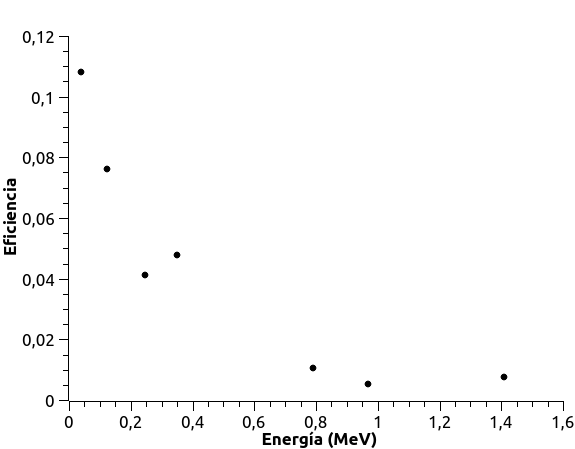
\includegraphics[width=0.7\linewidth]{6_1eficienciaenergia}
	\caption{Eficiencia según energía para el Eu$^{152}$}
	\label{fig:61eficienciaenergia}
\end{figure}

%%
%[Es igual la eficiencia del detector para todas las energías? ¿Cómo varía?]

Podemos ver como la eficiencia varía según la energía de forma exponencial, de modo que a menos energía, más eficiente es este detector, llegando a ser mínimamente eficiente para altas energías.



	
	\section{Medida de la resolución}
	
	Para obtener la resolución, dividimos la anchura del fotopico (FWHM) por su posición dentro de la escala de energía:
	
	\[R = \frac{\text{FWHM}}{\text{Posición del fotopico}}\times 100 \% = \frac{\Delta V}{V}\times 100 \% 
	\]
	
	
	
	\begin{figure}[H]
		
		\centering
		\begin{minipage}{0.45\textwidth}
			\centering
			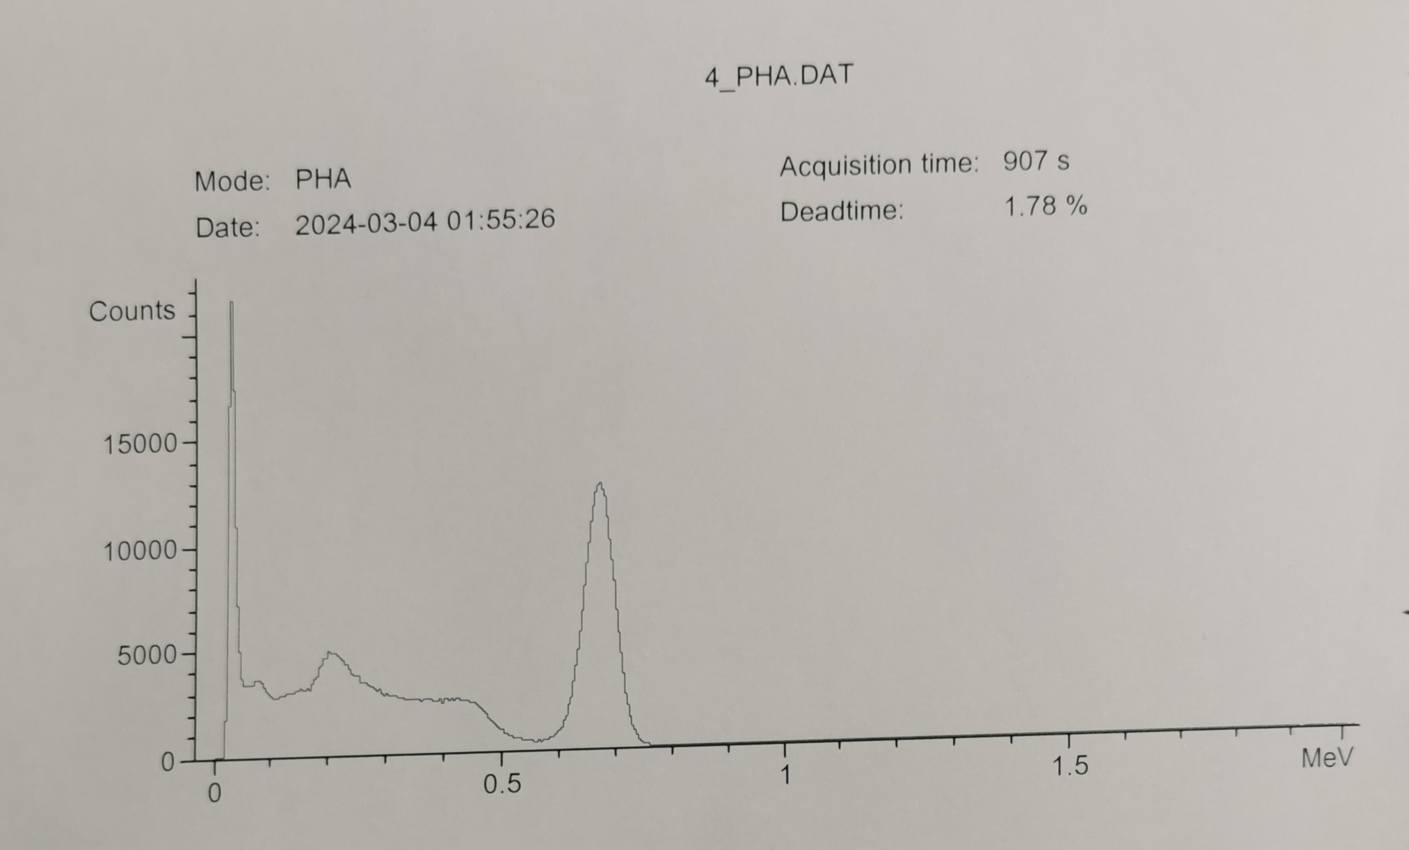
\includegraphics[width=1.1\linewidth]{../graficas_procesadas/PHA_4}
			\caption{Cesio-136}
			\label{fig:pha4}
		\end{minipage}\hfill
		\begin{minipage}{0.45\textwidth}
			\centering
			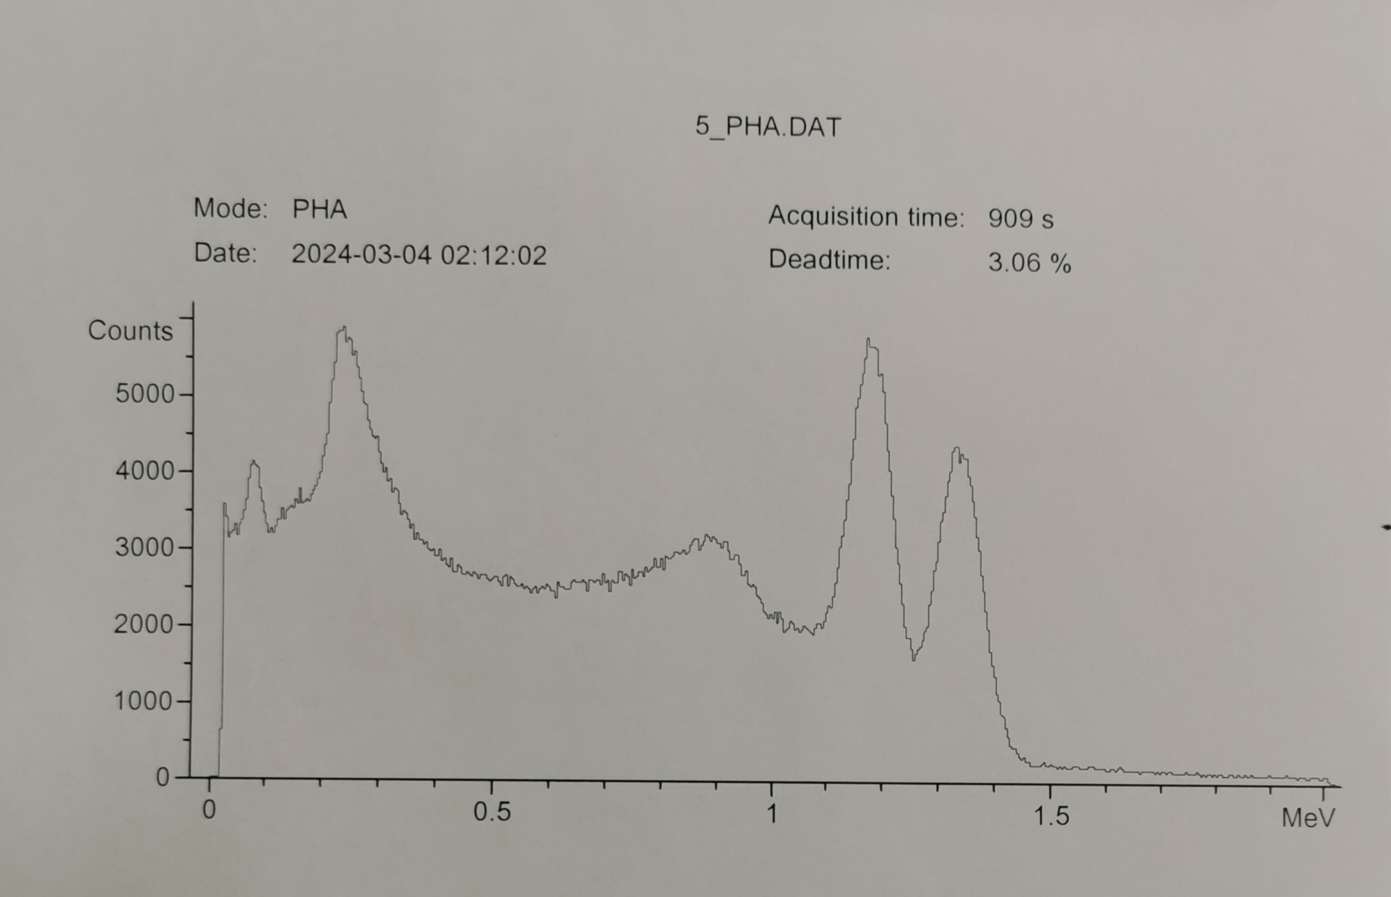
\includegraphics[width=1.1
			\linewidth]{../graficas_procesadas/PHA_5}
			\caption{Cobalto-60}
			\label{fig:pha5}
		\end{minipage}
		
		\begin{minipage}{0.45\textwidth}
			\centering
			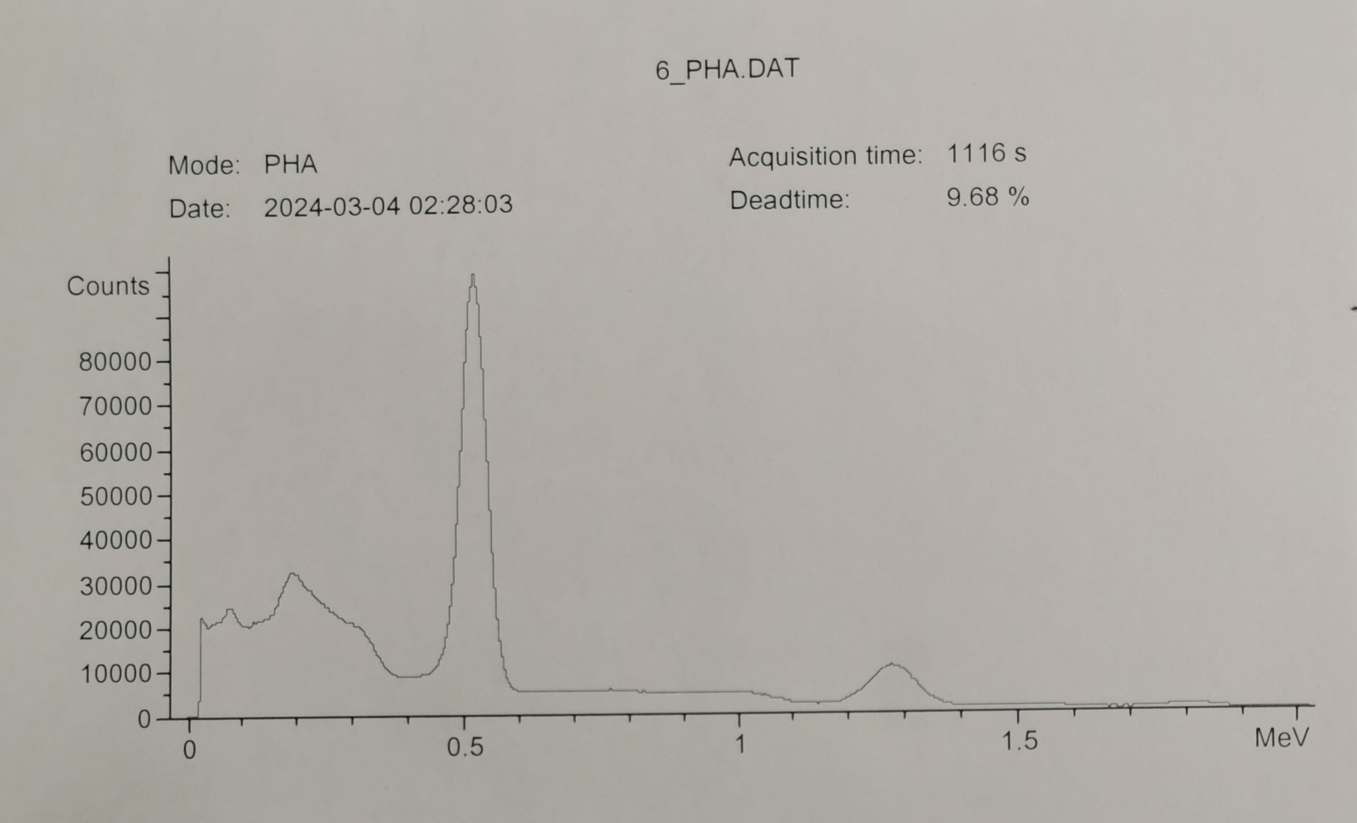
\includegraphics[width=1.1\linewidth]{../graficas_procesadas/PHA_6}
			\caption{Sodio-22}
			\label{fig:pha6}
		\end{minipage}\hfill
		\begin{minipage}{0.45\textwidth}
			\centering
			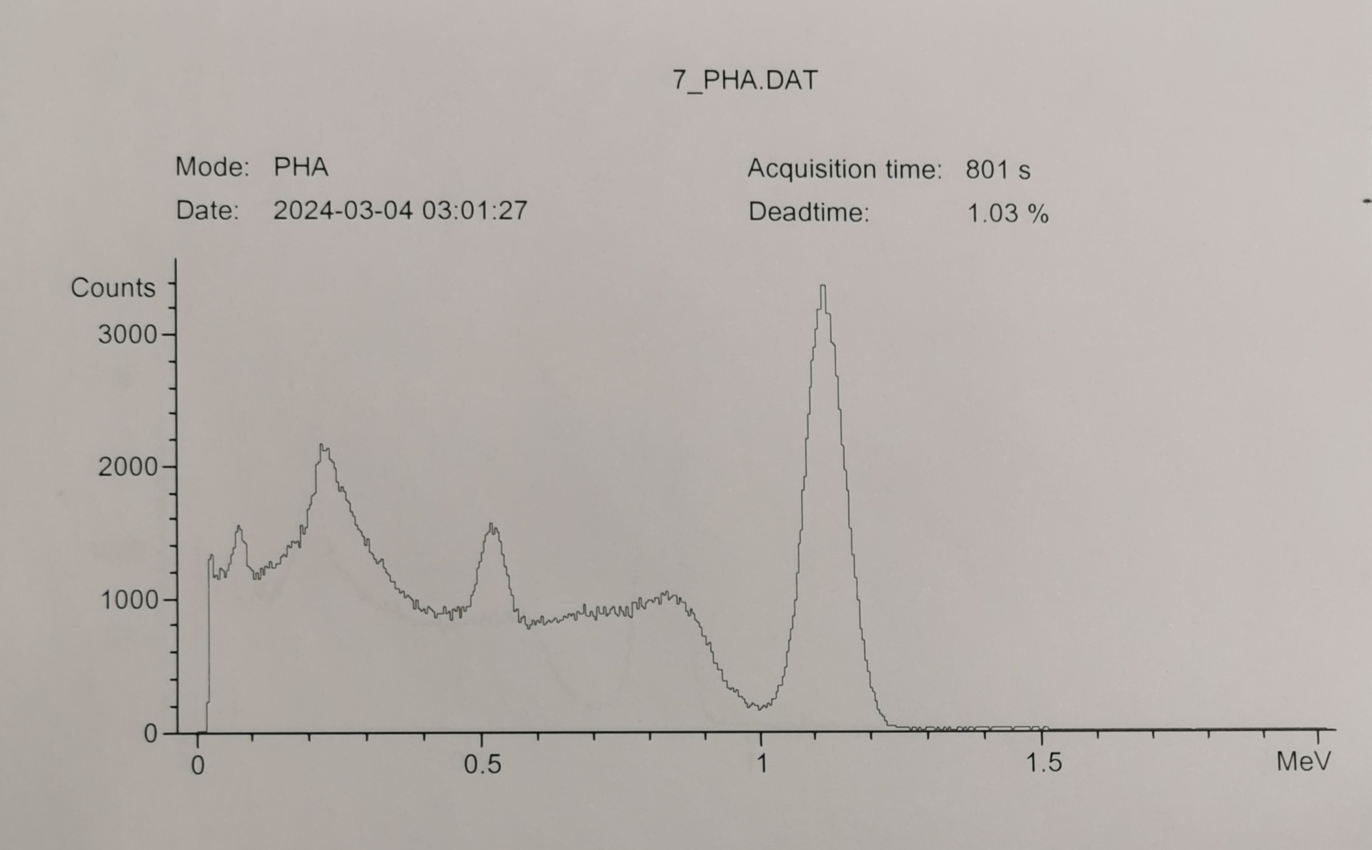
\includegraphics[width=1.1\linewidth]{../graficas_procesadas/PHA_7}
			\caption{Zinc-65}
			\label{fig:pha7}
		\end{minipage}
		
		\begin{minipage}{0.45\textwidth}
			\centering
			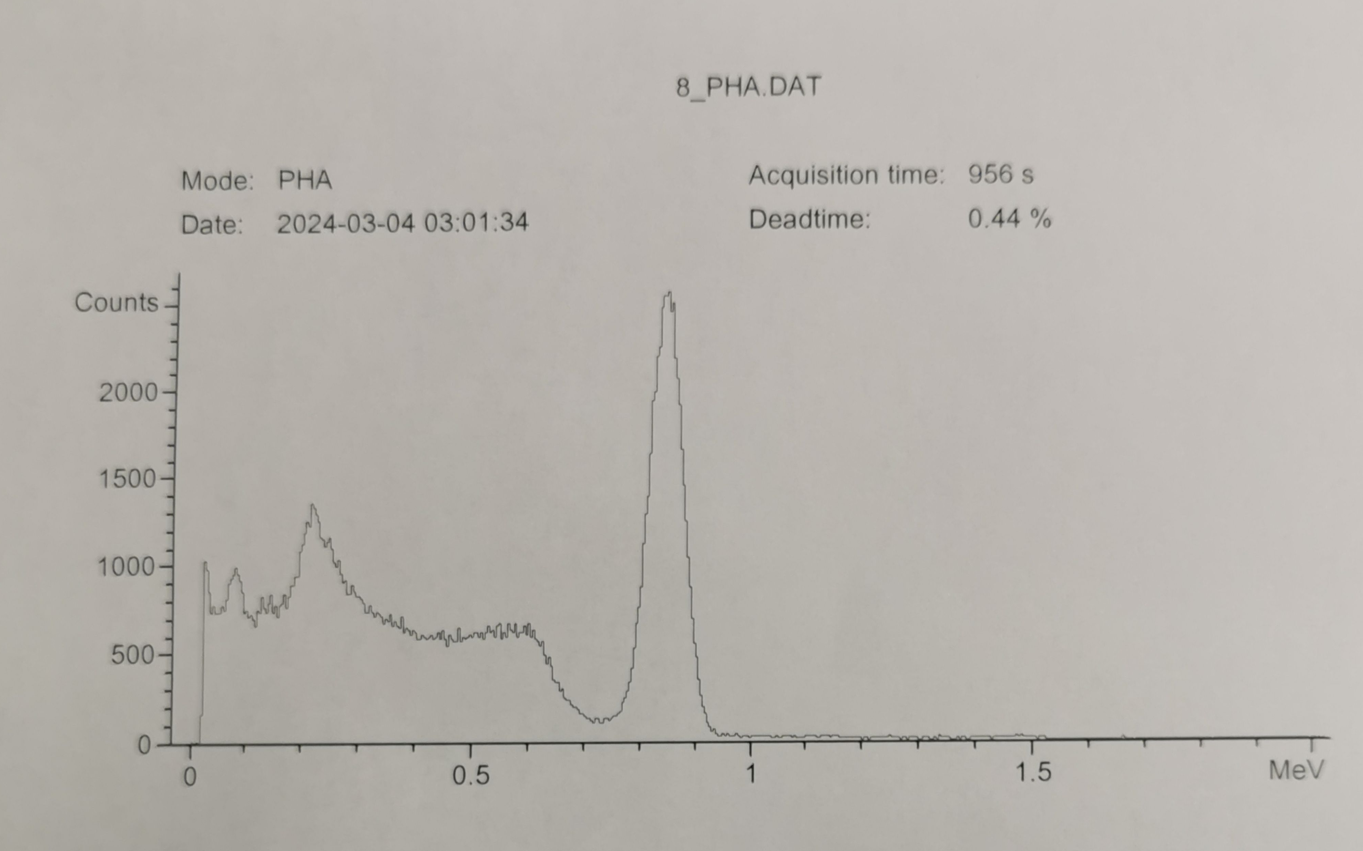
\includegraphics[width=1.1\linewidth]{../graficas_procesadas/PHA_8}
			\caption{Manganeso-54}
			\label{fig:pha8}
		\end{minipage}\hfill
		
	\end{figure}
	
	
	
	
	
	\begin{table}[H]
		\centering
		\begin{tabular}{|c|c|c|c|}
			\hline
			Fuente & Energía (MeV) & Anchura a semialtura & Resolución \\ \hline\hline
			Cs-137 & 0,669         & 0,056      & 8,37       \\ \hline
			Co-60  & 1,34          & 0,069      & 5,15       \\ \hline
			Co-60  & 1,175         & 0,066      & 5,62       \\ \hline
			Na-22  & 1,279         & 0,077      & 6,02       \\ \hline
			Na-22  & 0,518         & 0,051      & 9,85       \\ \hline
			Zn-65  & 1,122         & 0,077      & 6,86       \\ \hline
			Mn-54  & 0,846         & 0,064      & 7,57       \\ \hline
		\end{tabular}
	\caption{Resoluciones para distintos picos}
	\end{table}
	
	
\begin{figure}[H]
	\centering
	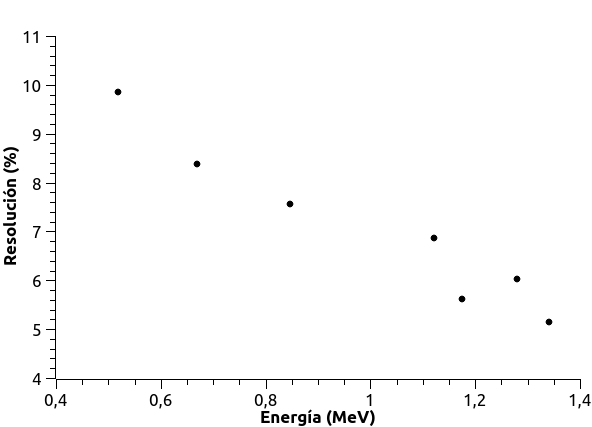
\includegraphics[width=0.7\linewidth]{6_2_resolucionenergia}
	\caption{Resolución según energía para los picos}
	\label{fig:62resolucionenergia}
\end{figure}


%%	
%[Es igual la resolución del detector para todas las energías?¿Cómo varía?]
En esta ocasión podemos ver como la resolución también se reduce con la energía, aunque de forma lineal, de modo que a bajas energías presenta una mayor resolución que a altas.





\vspace{\baselineskip}
	
	
	
	
	\section{Estudio de espectros}
	
	\subsection*{Cesio-137}
	
	\begin{itemize}
		\item Energía del borde Compton del espectro = 0,484 MeV
		\item Energía del borde Compton Teórica = 0,566 MeV
		\item Energía del pico de retrodispersión = 0,206 MeV
		\item Energía del pico de retrodispersión Teórica = 0,184 Mev
	\end{itemize}
	
	\subsection*{Cobalto-60}
	
	\begin{itemize}
		\item Energía del borde Compton del espectro = 0,970 MeV
		\item Energía del borde Compton Teórica = 0,994 MeV
		\item Energía del pico de retrodispersión = 0,235 MeV
		\item Energía del pico de retrodispersión Teórica = 0,214 MeV
	\end{itemize}
	
	
	\subsection*{Sodio-22}
	\begin{itemize}
		\item Energía del borde Compton del espectro = 1,08 MeV
		\item Energía del borde Compton Teórica = 0,962 MeV
		\item Energía del pico de retrodispersión = No se vé
		\item Energía del pico de retrodispersión Teórica = 0,213 MeV
	\end{itemize}
%0,962279546733151	0,212874959190336

	
	\subsection*{Zinc-65}
	\begin{itemize}
		\item Energía del borde Compton del espectro = 0,910 MeV
		\item Energía del borde Compton Teórica = 0,883 MeV
		\item Energía del pico de retrodispersión = 0,235 MeV
		\item Energía del pico de retrodispersión Teórica = 0,209 MeV
	\end{itemize}
	%0,882851766090748	0,208720888570405
	
	
	\subsection*{Manganeso-54}
	\begin{itemize}
		\item Energía del borde Compton del espectro = 0,652 MeV
		\item Energía del borde Compton Teórica = 0,693 MeV
		\item Energía del pico de retrodispersión = 0,219 MeV
		\item Energía del pico de retrodispersión Teórica = 0,196 MeV
	\end{itemize}
%	0,69292940431937	0,196019134396355
	
	%¿Se corresponden las energías del borde Compton y del pico de retrodispersión teóricas con las medidas por Ud?
	
	%%
	Vemos que las energías del borde Compton y del pico de retrodispersión teóricas son muy similares a las medidas.\\
	
	
	%cuestión_7
	El pico de 0,511 MeV en los espectros gamma de muestras radiactivas que emiten positrones se produce por la aniquilación de estos. 
	Cuando un positrón decae y se encuentra con un electrón en el material circundante, ambos se aniquilan mutuamente, convirtiendo su masa en energía en forma de dos fotones gamma de 0,511 MeV cada uno.\\
	
	%\vspace{\baselineskip}
	
	% cuestión 8
	
	El Zinc-65, sin embargo, presenta este pico sin ser emisor de positrones. Esto es debido a que al degradarse a Cobre-65, emite un rayo gamma de 1,114 MeV. Esta energía es superior a la requerida para la creación de un par electrón positrón (1,022 MeV), de modo que creará un positrón que después se aniquilará con un electrón libre del medio, resultando en el pico de aniquilación observado.\\
	
	%\vspace{\baselineskip}
	
	%cuestión 9
	
	También vemos en los espectros algunos picos resultantes de emisión de rayos X. Algunos de estos rayos son producidos por las interacciones con el plomo que recubre al detector, mientras que otros se emiten tras una conversión interna.\\
	% como el del cesio
	
	
	
	
	
	
	
	\section{Actividad desconocida}
	
	
	Disponemos de una muestra de Cobalto-60 con una actividad inicial en octubre de 2012 de 1$\si{\mu Ci}$, por lo que le corresponde una actividad corregida de 
	\[ A = A_0 \text{e}^{-\frac{\ln 2}{T_{1/2}}t} = 0,295\si{\mu Ci}
	\]
	
	\begin{figure}[H]
		\centering
		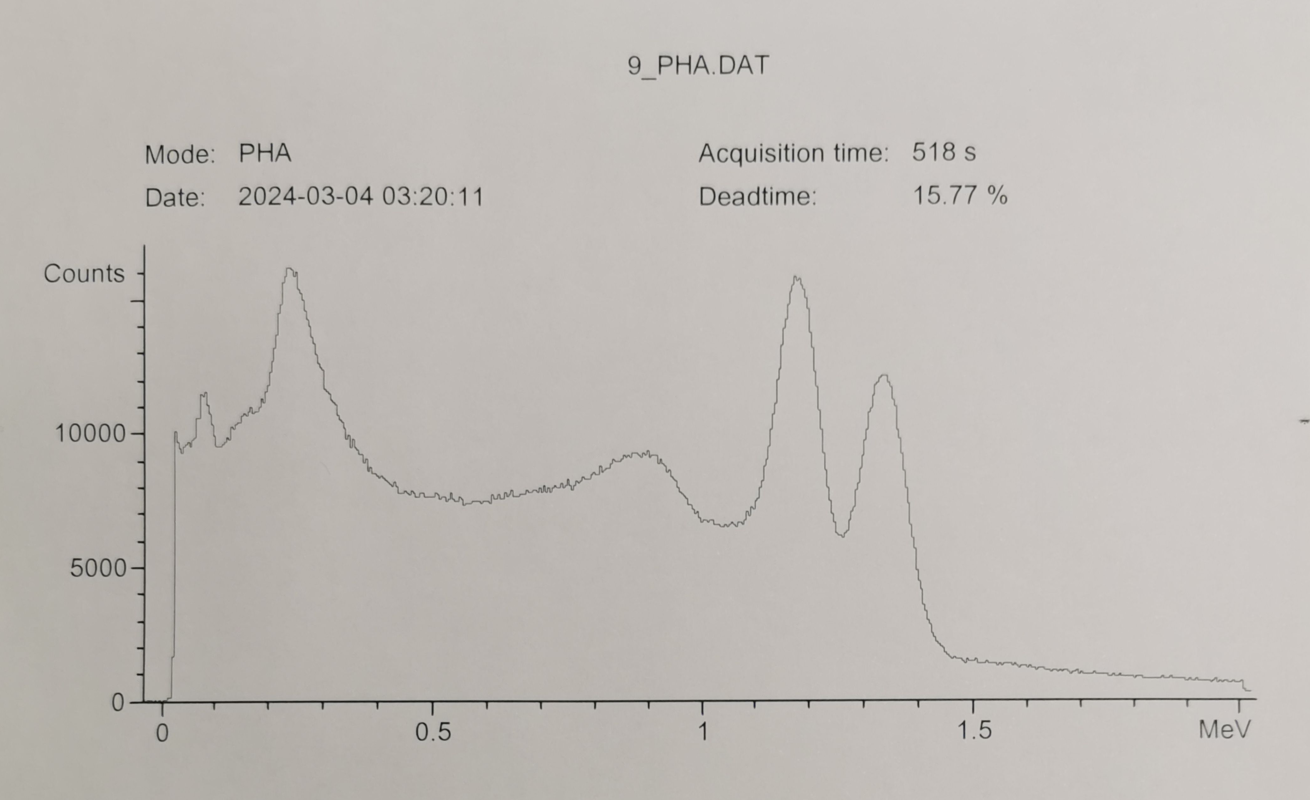
\includegraphics[width=0.7\linewidth]{../graficas_procesadas/PHA_9}
		\caption{Cobalto de actividad desconocida}
		\label{fig:pha9}
	\end{figure}
	
	Obtenemos las areas de los picos:
	\begin{itemize}
		\item Area 1er pico: 75,6 Bq
		\item Area 2o pico: 67,2 Bq
	\end{itemize}

	Media: 71,4 Bq
	
	\vspace{\baselineskip}
	
	Para la muestra de Cobalto-60 de actividad desconocida, realizamos la misma medida:
		\begin{itemize}
		\item Area 1er pico: 445
		\item Area 2o pico: 368
	\end{itemize}
	
	Media: 406,5 Bq
	
	\vspace{\baselineskip}
	
	Ahora podemos obtener la relación entre áreas de picos de la misma energía, que será la misma que la relación entre actividades radiactivas. Para ello usamos las energías medias:
	
	\[ \text{relación} = \frac{406,5}{71,4} = 5,69
	\]
	\[ \text{Actividad desconocida} = \text{relación} \times \text{actividad conocida}
	\]
	\[ \text{Actividad desconocida} = 0,295\si{\mu Ci} \cdot 5,69 = 1,68\si{\mu Ci}
	\]
	
	
	\section{Muestra desconocida}
	
	Tomamos el espectro de la muestra de elemento desconocido, recalibrando las energías y determinando los fotopicos.
	
	\begin{figure}[H]
		\centering
		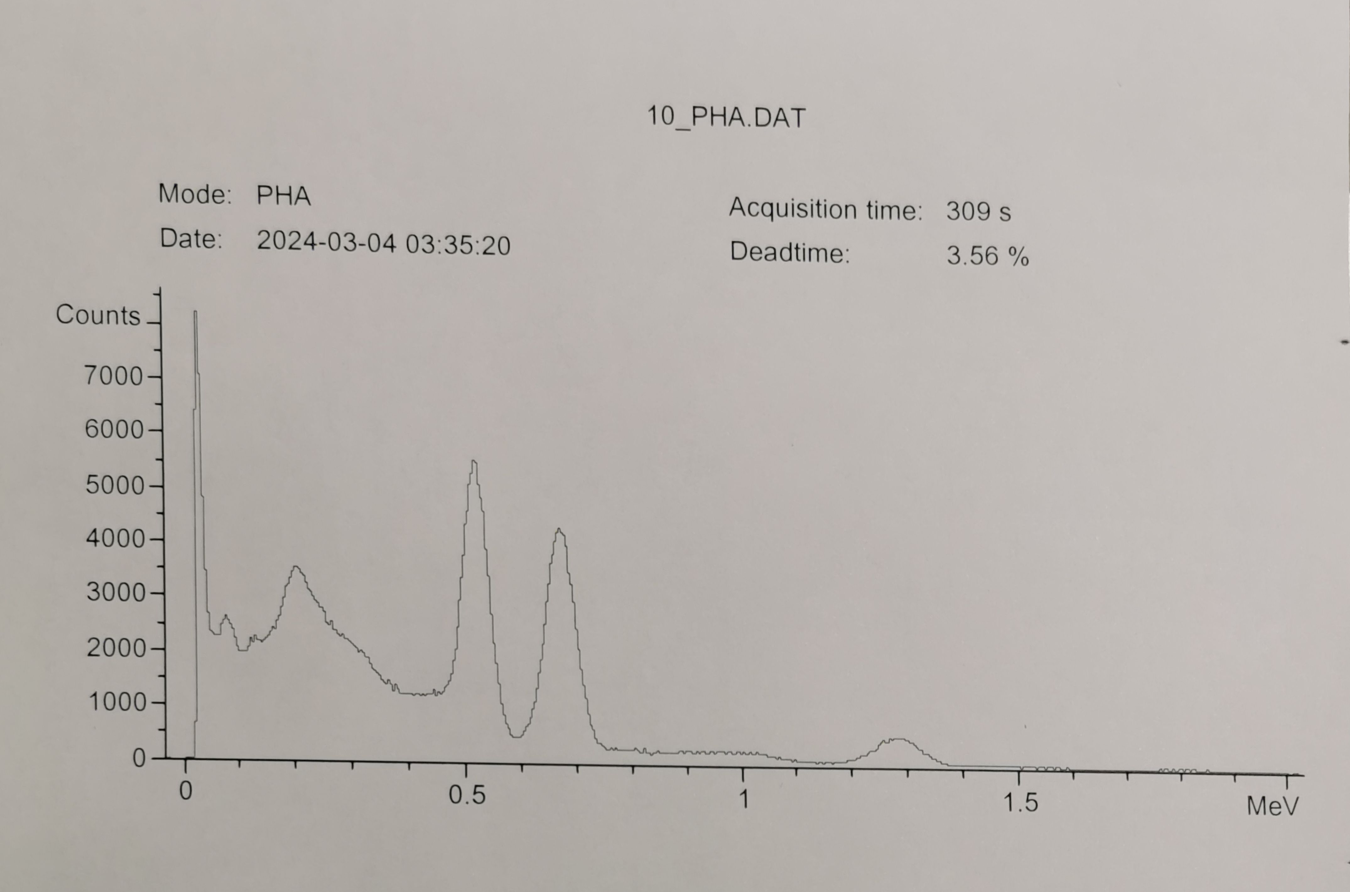
\includegraphics[width=0.7\linewidth]{../graficas_procesadas/PHA_10}
		\caption{Muestra de composición desconocida}
		\label{fig:pha10}
	\end{figure}
	
	
	Obtenemos 3 picos, de energías 
	\begin{itemize}
		\item Pico 1: 0,521 MeV
		\item Pico 2: 0,672 MeV
		\item Pico 3: 1,281 MeV
	\end{itemize}
	
	Observando los esquemas de desintegración, podemos identificar los picos del Cesio-137 (picos 1 y 2) y Sodio-22 (pico 3), por lo que estos deben ser los elementos que compongan la muestra.
	
	
	
	\section{Conclusión}
	
	
	Operando un detector INa(Tl), hemos tomado y estudiado los espectros de emisión gamma de distintos emisores, hemos observado el comportamiento en eficiencia y resolución del detector, y mediante comparaciones hemos podido deducir la actividad de una muestra y la composición de otra. \\
	
	La espectroscopia con estos detectores tiene un gran rango de aplicaciones por su capacidad para identificar y caracterizar materiales radiactivos, de modo que es ampliamente utilizada, por ejemplo, en medicina nuclear para estudiar la distribución de radiofármacos en el cuerpo, en geología para analizar la composición de muestras minerales o en control de calidad industrial para detectar contaminantes en productos.
	
	
	
\end{document}






